\section{Experiments}

To verify that the Discovery Service and the Specification retriever function correctly in real environment and on real machines, I set up a test bed depicted in figure ~\ref{fig:network-venn}.

 \begin{figure}[ht!]
\centering
  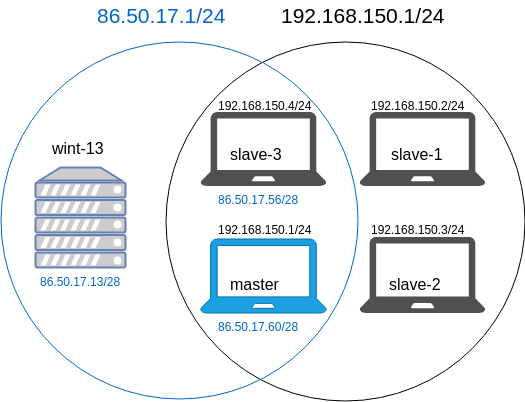
\includegraphics[width=12cm,height=12cm, keepaspectratio]{Network-venn.png}%
  \caption{The testbed hosts are located in a private network but master and slave-3 can also access internet via bastion host wint-13}
  \label{fig:network-venn}
\end{figure}

The testbed consist of a Lenovo Thinkpad T420S 4173L7G laptop computer with  4-core Intel i5-2540M CPU and 8 GB of RAM acting as a master node in the Cloudify cluster. The three slave-machines are Lenovo Thinkpad Edge E145's with 2-core AMD E1-2500 APU CPUs and 4 GB of RAM. The master host has Centos 7 installed as the operating system to accommodate Cloudify's installation requirements. The three slave machines are running Ubuntu 16.04 as the OS of the slaves can be anything as long as they are Linux-based and the hosts themselves can be accessed via SSH.

As seen on figure ~\ref{fig:network-venn}, the testbed setup has two different networks. The Master can be accessed remotely via a bastion host \textit{wint-13}. Wint-13 itself
